\documentclass[11pt]{jarticle}
\usepackage{latexsym}
\usepackage{mathrsfs}
\usepackage{amssymb}
%\usepackage{url}
%\usepackage{lscape}
\usepackage[dvipdfmx]{graphicx}
\usepackage{theorem}

%% for apple LaserWriter Series %%
%% 
\setlength{\topmargin}{-0.5in}
\setlength{\textwidth}{5.6in}
\setlength{\textheight}{8.8in}
\setlength{\oddsidemargin}{0.35in}
\setlength{\evensidemargin}{0in}

\usepackage{theorem}
\renewcommand{\baselinestretch}{1.25}
\setlength{\parskip}{0.25ex}
\renewcommand{\arraystretch}{0.85}
\begin{document}

\section{目的}

自動車のカーナビゲーションシステム,スマートフォンのロガーアプリ等で得られる地上座標の移動履歴が蓄積されたときに,
一連の移動履歴あるいはその部分を比較や検索が可能なデータとして扱えるようにするための類似性を定義し,
類似性に基づく類似度計算,照合を行うアルゴリズムを設計し,計算実験を行ってアプリケーションと問題点を検討する.

\section{定義}

\subsection{位置点}
位置点は,地表上の緯度と経度の組 $(a, b) \in \mathbb{Q}^2$ (ただし $-90 \leq a \leq 90$, $-180 < b \leq 180$)である.
位置点の得られた時刻に関して真に昇順となっている列(時系列) $P = ((a_0, b_0), \ldots,(a_{n-1}, b_{n-1}))$ を軌跡 trajectory とよぶ.

現実には,
GPS では位置情報が時刻(UTC),地球上での緯度 latitude,経度 longitude の 3 つ組として得られ,ログはいくつかの一般的な形式でこれらが記録,保存される.
ここでは,列において位置点は時刻に関して真に昇順で並ぶものとして,時刻を省略する.
同様に,付加情報として標高,対地速度が情報として得られることもあるが,これらはとりあえず無視して考える.

\subsection{2 点を同一地点とみなす距離}
現実に得られる位置点の座標は,移動での変化のほか,
GPS の技術に起因する測量誤差,車線や上下線の違いなどで生じる道路の幅程度の距離の差,鉄道の線番の違いによる差など,意味的には同一地点とみなしてよいが,座標値としては異なる違いも生じる.
これに相当する距離の程度は,利用目的やデータソースなどに依存しケースバイケースになるであろうが,たとえば人の徒歩から自動車あるいは鉄道での移動について,およそ 30 秒おきに座標を得ることができるならば,数十メートルから数百メートルで考えることができる.
この同一地点とみなせる距離の最大値を $\delta > 0$ で表し,距離がこの閾値内であれば,同じ位置にあるとみなすことにする.
($\delta$ の大きさとその妥当性については,計算実験をふまえ議論する.とりあえず 50m から 500m と考えてよい.)

\subsection{2 位置点間の距離}
位置点の組 $p, q$ が与えられたとき,これらが同一地点であるかを判定,あるいは移動中の二点間の軌跡を推定するといった目的のために,
地表上での距離を求めたい.
ここでは,位置点の高度(標高)は無視できるものとして,地球を楕円体で近似し距離を求める.
ヒュベニの公式 \cite{amano-tec,GSI,Hubeny-formula-ref1,Hubeny-formula-ref2} で高次の項のみを使い $p=(p_a, p_b), q=(q_a, q_b)$ 間の距離 $d(p,q)$ を次のように求める:
\[
d(p,q) = \sqrt{(|p_a - q_a|\cdot M)^2 + \left(|p_b - q_g\b|\cdot N\cos{P} \right)^2} \,,
\]
ただし緯度,経度の単位はラジアン rad であり,$P = \frac{p_a+q_a}{2}$ (緯度の平均値), $M$ は地球(楕円体)の子午線曲率半径,$N$ は同じく卯酉線曲率半径で,
地球の赤道半径 $R_x$,極半径 $R_y$,第1離心率 $e=\sqrt{\frac{R_x^2 - R_y^2}{R_x^2}}$ から,$W = \sqrt{1 - (w^2 \cdot \sin P)^2}$ とおくと
\begin{eqnarray*}
M &=& \frac{Rx\cdot (1 - e^2)}{W^3} \,, \\
N &=& \frac{Rx}{W}
\end{eqnarray*}
である.

\subsection{位置点と2点間の距離}

二つの移動履歴をあらわす点列は,どちらも移動速度に対して十分に測定と記録の頻度が高い,あるいは交差点や駅など停止したり速度が落ちる地点が一致するならば,
$\delta$近傍にあり同一地点とみなせる組の数を最大化することで,文字列の最大共通部分列 longest common subsequence の考え方で,共通部分を抽出することができる.
しかし,どちらか一方,あるいは両方の移動履歴がそうでない場合,移動履歴の軌跡としてほぼ一致しても,座標点の多くに一致する点が存在しない可能性がある.
二つの移動履歴で二点間の線分が一致する場合も,
位置点の距離が広ければ,より類似度が高いと考えることもできるが,二点間の軌跡を直線として推定するのは乱暴ということになる.

そこで,点列 $P, Q$ がある場合に,
\begin{itemize}
\item[(1)] $P$ の位置点 $p_i$ と $Q$ の位置点 $q_j$ が同一視できる $d(p_i, q_j) \leq \delta$ か,
\item[(2)] $P$ の位置点 $p_i$ と $Q$ の連続する 2 つの位置点 $q_j, q_{j+1}$ を結ぶ線分との距離 $d(p_i, (q_j, q_{j+1}))$ が $\delta$ 以内,
\item[(3)] (2) の逆,$Q$ の位置点 $q_j$ と $P$ の 2 位置点 $p_i, p_{i+1}$ の線分の距離 $d((p_i, p_{i+1}), q_j)$ が $\delta$ 以内,
\end{itemize}
であるときに,位置点が一致,あるいは位置点に対し一致する距離内を移動したとみなし,
(1) の場合の一致度を $1$, (2) および (2) の場合の一致度を $\frac{1}{2}$ とし,
$P$ と $Q$ の間で一致度の総和を最大化する添え字の組の列で得られる,その最大値を $P, Q$ の類似度とする.
$P$ の点の線分と $Q$ の点の線分の交差や接近は,類似度に寄与しないものとする.

\begin{figure}[h]
\centering
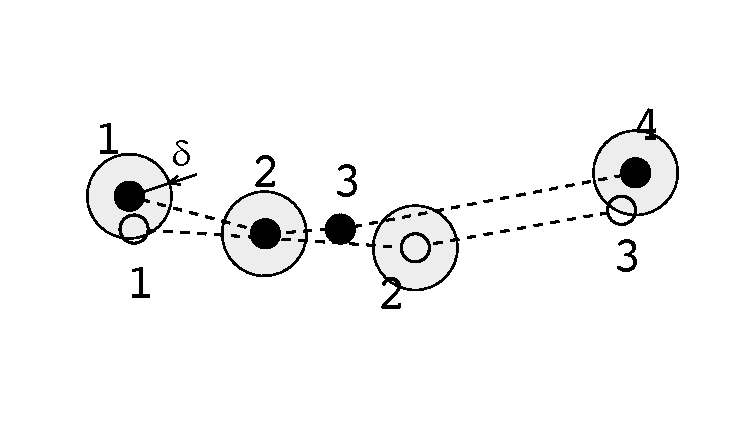
\includegraphics[scale=0.5]{matching.pdf}
%\caption{$G_1$}\label{fig:g_1}
\end{figure}

位置点列 $P=(p_0, \ldots, p_{m-1})$ の位置点と,隣り合う位置点の間で定義される線分,が交互に並ぶ列
\[
\hat{P} = \langle p_0, (p_0, p_1), p_1, (p_1, p_2), \ldots, (p_{m-2}, p_{m-1}), p_{m-1} \rangle
\]
を経路 path という.
その要素 $\hat{P}(i)$ ($0 \leq i \leq 2m-1$) を
\[
\hat{P}(i) = \left\{
\begin{array}{ll}
p_{i/2} & \mbox{$i$ is even}\\
(p_{(i-1)/2}, p_{(i-1)/2 + 1}) & \mbox{$i$ is odd}
\end{array}
\right.
\]
と書くとする. 

位置点列 $P = (p_0, \ldots, p_{m-1})$ と $Q = (q_0, \ldots, q_{n-1})$ について,それぞれの経路 $\hat{P}, \hat{Q}$ の添え字の組の列
$\psi = \langle (\psi_0(0), \psi_1(0)), \ldots, (\psi_0(k-1), \psi_1(k-1)) \rangle$ で
\begin{enumerate}
%\item $k \leq \min(m,n)$, 
\item $0 \leq \psi_0(0) < \cdots < \psi_0(k-1) \leq m-1$ および $0 \leq \psi_1(0) < \cdots < \psi_1(k-1) \leq n-1$,
\item すべての $0 \leq i \leq k-1$ について $\psi_0(i)$ または $\psi_1(i)$, またはその両方が奇数(単独の位置点),かつ
\item $d(\hat{P}(\psi_0(i)), \hat{P}(\psi_1(i)) \leq \delta$,  
\end{enumerate}
であるとき,$\psi$ を位置点列 $P$ と $Q$ の$\delta$ 近接部分列($\delta$-proximity subsequence)であるという.
$P, Q$ の $\delta$-ps $\psi$ の類似長 similarity length $|\psi|$ は,$\psi$ の組のうち奇数のみの組の数とそれ以外の数の $\frac{1}{2}$ の和である.
$P, Q$ の $\delta$-ps の中で,その類似長が最大のものを,$P, Q$ の最長 $\delta$近接部分列 $\delta$-lps とよび,その類似長を $P$ と $Q$ の類似度という.


\begin{defn}[2つの位置点列の最長共通部分列 (II)]
軌跡 $q$ の位置点および位置点と次の点の間の線分からなる列
\[
\tilde{q} = (r_1, (r_1, r_2), r_2, (r_2, r_3), r_3, \ldots, r_{n-1}, (r_{n-1}, r_n), r_n)
\]
を $q$ の経路 path という.
ある正の値 $\varepsilon \in \mathbb{R}^+$ について,
二つの位置点列 $q = (s_1, \ldots, s_n)$ と $r = (t_1, \ldots, t_p)$ それぞれの経路 $\tilde{q}, \tilde{r}$ の間の $\varepsilon$共通部分列とは,
 $\tilde{q}$ と $\tilde{r}$ の (1) 点と点の距離が $\varepsilon$ 以内,または (2) 点と線分の距離が $\varepsilon$ 以内である対を等しいとみなした最長共通部分列 longest common super sequence である.
\end{defn}

\begin{example}
例をつくってみよう.
\end{example}

\begin{thebibliography}{4}

\bibitem{amano-tec}
アマノ技研ウェブページ
\newblock  {\tt https://amano-tec.com/apps/paceruler.html}

\bibitem{toriaezu}
ヒュベニの公式
\newblock {\tt http://hp.vector.co.jp/authors/VA002244/yacht/geo.htm}

\bibitem{GSI}
国土地理院ウェブページ ``測量計算(測量計算サイト/距離と方位角の計算)''
\newblock {\tt https://vldb.gsi.go.jp/sokuchi/surveycalc/main.html}

\bibitem{Hubeny-formula-ref1}
K. Hubeny: 
\newblock Weiterentwicklung der Gauss'schen Mittelbreitenformeln, Z.Vermess, {\bf 84}, 159-163, 1959.

\bibitem{Hubeny-formula-ref2}
K. Hubeny: 
\newblock
Zur Entwicklung der Gauss'schen Mittelbreitenformeln. Osterreichische Zeitschrift fur Vernessubgswesen, {\bf 42} Jahrgang (1954) Nr.1,S. 8-17

\end{thebibliography}

\end{document}
